\documentclass[10pt,a4paper]{article}
%\documentclass[aps,prl]{revtex4-1}
\usepackage[margin=2.5cm,footskip=1.cm,includefoot]{geometry}% spremenimo sirine robov
\usepackage{floatrow}
\usepackage{hyperref}
\usepackage{amsmath}
\usepackage{fullpage}
\usepackage{amsfonts}
\usepackage{amssymb}
\usepackage{lmodern}
\usepackage{url}
\usepackage[labelformat=simple,font=small]{subcaption}
\usepackage[font=small]{caption}
%\usepackage{subcaption}
\usepackage[multiple]{footmisc}
\usepackage[]{units}
\usepackage{bm}
\usepackage{fancyhdr}
%\usepackage[demo]{graphicx}
\usepackage{graphicx}
\usepackage{mhchem}
\newcommand{\iu}{{i\mkern1mu}}

\addtolength\hoffset{0.5cm}%horizontalni premik
%vse pametne funkcije ki jih lahko rabimo (lahko tudi kopiras direktno zraven)
\setlength{\parindent}{0pt}%ni pomika za paragrafe
\setlength{\parskip}{0.75ex}%med paragrafi je malo lufta

\usepackage[pdftex]{graphicx}%za slike: predvidimo da bomo klicali pdflatex.

\usepackage{amsmath}
\usepackage{amsfonts}
\usepackage{mathrsfs}
\usepackage[usenames]{color}
\usepackage[slovene]{babel}
\usepackage[utf8]{inputenc}%to omogoca uporabo sumnikov. Brez tega rabis \v{c}, \v{s}, \v{z} in vse ostalo.

%nekaj koristnih funkcij.
\newcommand{\HRule}{\rule{\linewidth}{0.5mm}}   %debela črta čez celo stran

\newcommand{\ve}[1]{\ensuremath{\mathbf{#1}}} % for vectors
\newcommand{\gv}[1]{\ensuremath{\mbox{\boldmath$ #1 $}}} 
% for vectors of Greek letters
\newcommand{\uv}[1]{\ensuremath{\mathbf{\hat{#1}}}} % for unit vector
\newcommand{\abs}[1]{\left| #1 \right|} % for absolute value

\renewcommand{\Re}{\mathop{\rm Re}}
\renewcommand{\Im}{\mathop{\rm Im}}
\newcommand{\Tr}{\mathop{\rm Tr}}
\newcommand{\dd}{\,\mathrm{d}}
\newcommand{\ddd}{\mathrm{d}}
\newcommand{\ii}{\mathrm{i}}
\newcommand{\lag}{\mathcal{L}\!}
\newcommand{\ham}{\mathcal{H}\!}
\newcommand{\four}[1]{\mathcal{F}\!\left(#1\right)}
\newcommand{\bigO}[1]{\mathcal{O}\!\left(#1\right)}
\newcommand{\sh}{\mathop{\rm sinh}}
\newcommand{\ch}{\mathop{\rm cosh}}
\renewcommand{\th}{\mathop{\rm tanh}}
\newcommand{\erf}{\mathop{\rm erf}}
\newcommand{\erfc}{\mathop{\rm erfc}}
\newcommand{\sinc}{\mathop{\rm sinc}}
\newcommand{\rect}{\mathop{\rm rect}}
\newcommand{\ee}[1]{\cdot 10^{#1}}
\newcommand{\inv}[1]{\left(#1\right)^{-1}}
\newcommand{\invf}[1]{\frac{1}{#1}}
\newcommand{\sqr}[1]{\left(#1\right)^2}
\newcommand{\half}{\frac{1}{2}}
\newcommand{\thalf}{\tfrac{1}{2}}
\newcommand{\pd}{\partial}
\newcommand{\Dd}[3][{}]{\frac{\ddd^{#1} #2}{\ddd #3^{#1}}}
\newcommand{\DD}[3][{}]{\frac{D^{#1} #2}{D #3^{#1}}}
\newcommand{\Pd}[3][{}]{\frac{\pd^{#1} #2}{\pd #3^{#1}}}
\newcommand{\bra}[1]{\langle #1 \vert}
\newcommand{\ket}[1]{\vert#1\rangle}
\newcommand{\avg}[1]{\left\langle#1\right\rangle}
\newcommand{\norm}[1]{\left\Vert #1 \right\Vert}
\newcommand{\braket}[2]{\left\langle #1 \vert#2 \right\rangle}
\newcommand{\obraket}[3]{\left\langle #1 \vert #2 \vert #3 \right \rangle}
\newcommand{\en}[1]{\mathop{\rm #1}}
\newcommand{\hex}[1]{\texttt{0x#1}}

\renewcommand{\iint}{\mathop{\int\mkern-13mu\int}}
\renewcommand{\iiint}{\mathop{\int\mkern-13mu\int\mkern-13mu\int}}
\newcommand{\oiint}{\mathop{{\int\mkern-15mu\int}\mkern-21mu\raisebox{0.3ex}{$\bigcirc$}}}

\newcommand{\wunderbrace}[2]{\vphantom{#1}\smash{\underbrace{#1}_{#2}}}


\renewcommand{\vec}[1]{\overset{\smash{\hbox{\raise -0.42ex\hbox{$\scriptscriptstyle\rightharpoonup$}}}}{#1}}
\newcommand{\bec}[1]{\mathbf{#1}}

%\pagestyle{plain}
\pagestyle{headings}

\usepackage{titlesec}
\usepackage{cleveref}
\renewcommand{\thesubfigure}{(\alph{subfigure})}
\captionsetup[sub]{labelformat=simple}

\titleformat*{\section}{\Large\bfseries}
\titleformat*{\subsection}{\large\bfseries}
\titleformat*{\subsubsection}{\large\bfseries}
\titleformat*{\paragraph}{\large\bfseries}
\titleformat*{\subparagraph}{\large\bfseries}

\usepackage{color}

\pagenumbering{arabic}

\begin{document}
%%% NASLOVNA STRAN


\begin{center}

% 
\includegraphics[width=0.35\textwidth]{logo_fmf_uni-lj_en.pdf}\\[8ex] 

\vspace{3mm}


%{\large }\\
\vspace{2 cm}

{ \Large }Magistrsko delo\\             
\vspace{3cm}


{\large Avtor: Jan Šuntajs\\
\large Mentor: dr. Janez Bonča \\
\large Mentor: doc. Lev Vidmar 
\vspace{2cm}



Ljubljana, 2017}
\vfill
\begin{abstract}

\end{abstract}

\end{center}

\cleardoublepage

\thispagestyle{empty}


%\tableofcontents
\clearpage
\pagestyle{fancy}
\fancyhf{}
\cfoot{\thepage}
\setcounter{page}{1}

\section{Uvod}
%VIRI: NANDKISHORE, HUSE, UVOD
%ABANIN, UVOD
%MONDAINI, RIGOL (za stil pisanja pri nanašanju na Andersona)
Nastop \emph{večdelčne lokalizacije} (ang. \emph{many-body localization}, v nadaljevanju MBL) v izoliranih neurejenih kvantnomehanskih sistemih s prisotnostjo meddelčnih interakcij vodi do osupljivih lastnosti tovrstnih sistemov. Med njimi je poglavitna in najočitnejša odsotnost termalizacije, sicer značilne za generične večdelčne sisteme z ergodično dinamiko. V termodinamski limiti unitaren dolgočasovni razvoj poljubnih začetnih stanj ergodičnih sistemov vodi do ravnovesja, v katerem pričakovane vrednosti kvantnomehanskih opazljivk podajajo ustrezna kvantnomehanska ansambelska povprečja. Zaradi odsotnosti sklopitve z zunanjim rezervoarjem je tovrstna relaksacija neravnovesnih začetnih stanj proti ravnovesnim termalnim vrednostim v izoliranem sistemu možna le, če sistem sam sebi predstavlja `efektivno toplotno kopel'. To pomeni, da se mora podsistem z makroskopsko zanemarljivim deležem prostostnih stopenj  celotnega sistema s preostankom sistema sklapljati podobno, kot se v običajni formulaciji statističnomehanskih ansamblov sistemi sklapljajo z zunanjim rezervoarjem~\cite{abanin2018ergodicity}~\cite{nandkishore2015many}. \\
\begin{minipage}[t]{0.42\textwidth}
\noindent \\
Skupaj z integrabilnimi sistemi predstavljajo MBL sistemi pomemben protiprimer
zgoraj opisani dinamiki ergodičnih sistemov, kar je shematsko predstavljeno na Sliki~\ref{fig:abanin_thermalization}. Prikazan je časovni razvoj netipičnega začetnega profila kvantnomehanske opazljivke, točneje gostote delcev, v ergodičnem in MBL primeru. Medtem ko pri prvem pričakovane vrednosti lokalnih opazljivk po dolgem času določajo vrednosti ansambelskih povprečij, ki so odvisne le od nekaj dobro definiranih makroskopskih količin, denimo energije in števila delcev, je obnašanje MBL sistemov popolnoma drugačno. `Spomin' na netipičnost začetne konfiguracije se namreč v pričakovanih vrednostih lokalnih opazljivk ohrani tudi po 
\end{minipage}\hfill
\begin{minipage}[t]{0.55\textwidth}
\begin{figure}[H]
\centering{
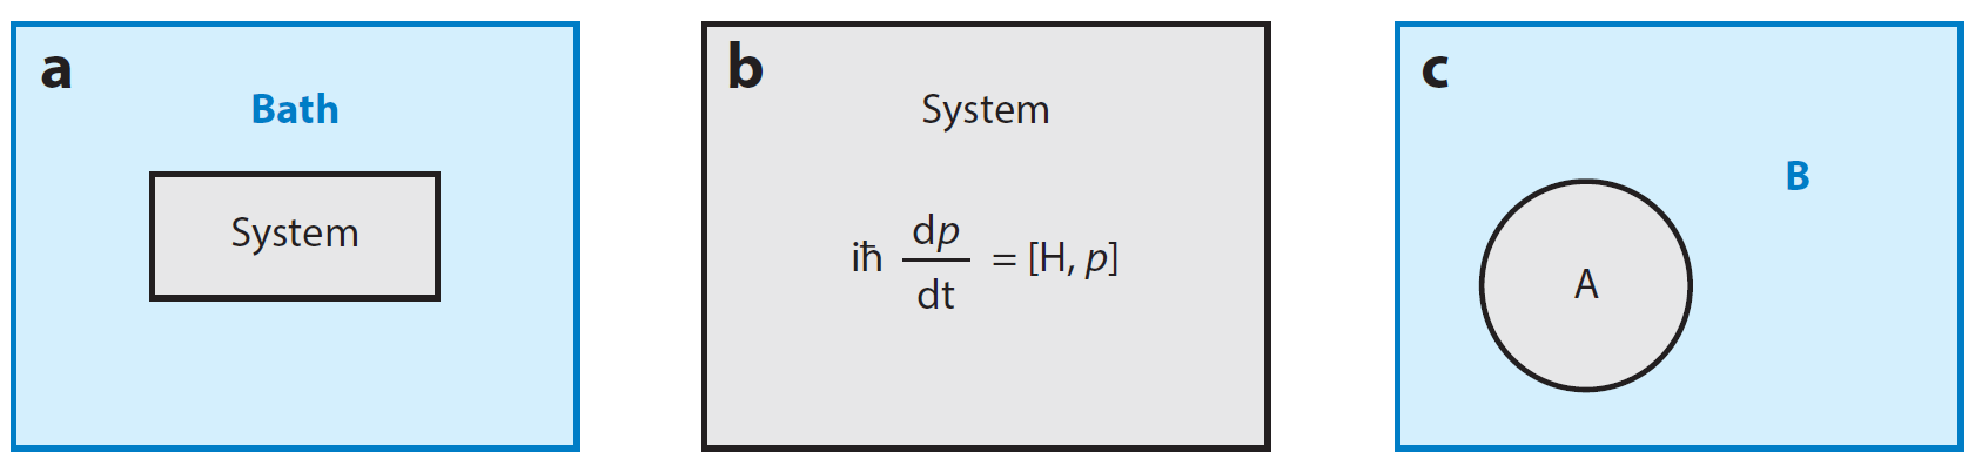
\includegraphics[width=1\textwidth]{nandkishore_huse_reservoir.pdf}}
\caption{
\textbf{a)} Pri običajnem kvantnostatističnem opisu sistema privzamemo njegovo sklopitev z zunanjim rezervoarjem, s katerim lahko izmenjuje denimo energijo in delce. \textbf{b)} Tu obravnavamo zaprte oziroma izolirane kvantne sisteme, katerih dinamiko določa unitaren časovni razvoj začetnih stanj. \textbf{c)} Pri obravnavi termalizacije v zaprtih kvantnih sistemih je smiselno sistem razdeliti na podsistema A in B, pri čemer je v A makroskopsko zanemarljiv delež prostostnih stopenj celotnega sistema. V kolikor večji podsistem B manjšemu podsistemu služi kot toplotni rezervoar, je termalizacija možna tudi v zaprtem kvantnem sistemu. Slika je bila vzeta iz Ref.~\cite{nandkishore2015many}. 
}
\label{fig:abanin_thermalization}
\end{figure}
\end{minipage}
dolgočasovnem razvoju. Ker termalizacija poteka prek izmenjave delcev in energije med različnimi deli ergodičnega
sistema, torej preko različnih transportnih mehanizmov, so, v nasprotju s tipično prevodnimi termalizirajočimi sistemi, lokalizirani sistemi izolatorji. V neurejenih sistemih \emph{neinteragirajočih} delcev \\
\begin{minipage}[t]{0.42\textwidth}
\noindent 
je tovrstno
obnašanje dobro poznano~\cite{lagendijk2009fifty}~\cite{abrahams201050} in dolgo preučevano, saj je P.W. Anderson v svojem prelomnem članku~\cite{anderson1958absence} že leta 1958 pojasnil vlogo nereda pri prehodu med prevodnim 
in izolativnim obnašanjem v preprostem modelu tesne vezi ob prisotnosti naključnih potencialov. Omenjeni mehanizem zloma ergodičnosti v neinteragirajočih sistemih danes imenujemo \emph{Andersonova lokalizacija}, sistemi, v katerih je realiziran, pa so Andersonovi izolatorji. Ob dovolj močnem potencialnem neredu so vse enodelčne valovne funkcije tovrstnih sistemov lokalizirane, pri čemer njihova verjetnostna gostota pojema eksponentno z razadaljo od neke točke v prostoru. V nasprotju s prostorsko razsežnimi valovnimi funkcijami lokalizirane 
\end{minipage}\hfill
\begin{minipage}[t]{0.55\textwidth}
\begin{figure}[H]
\centering{
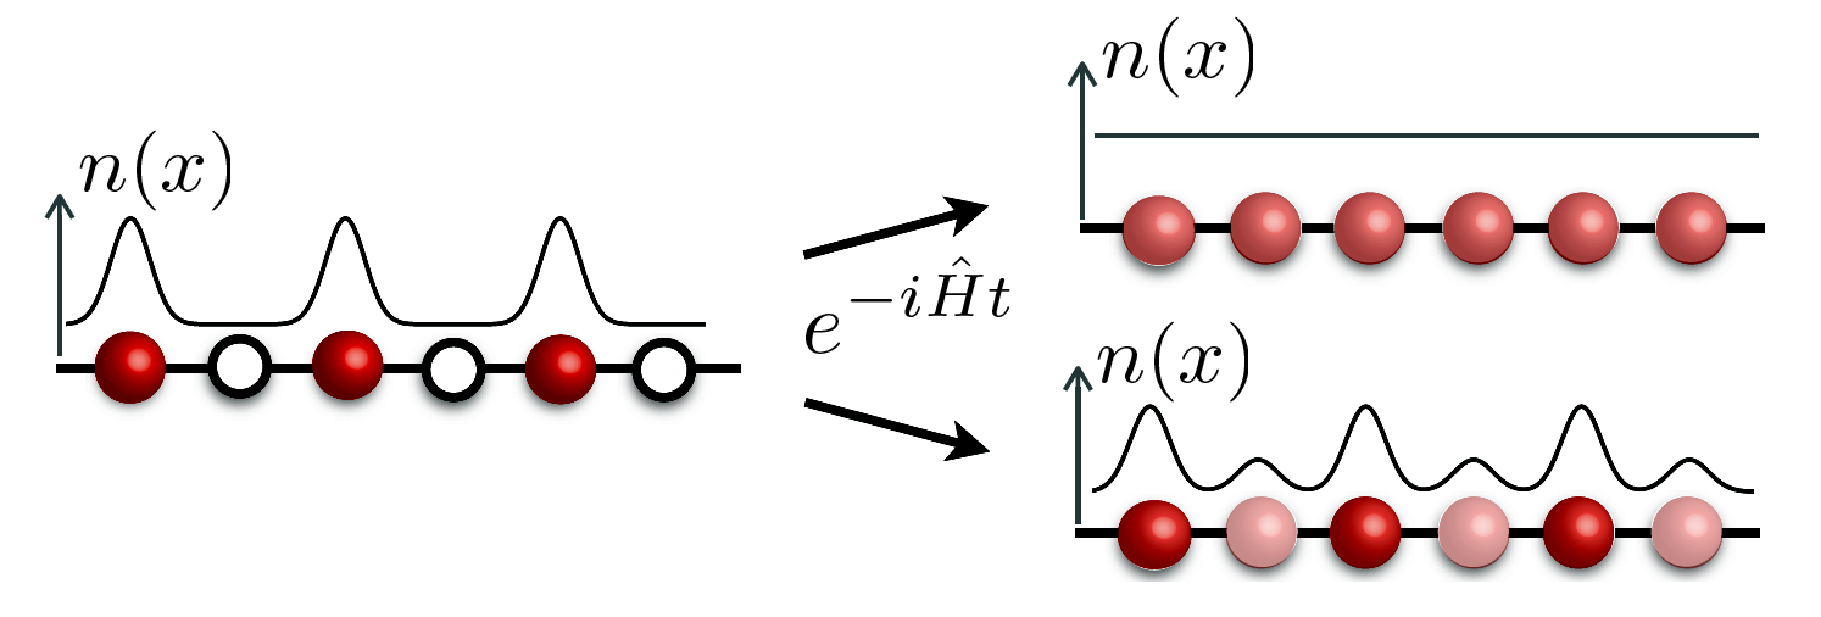
\includegraphics[width=0.95\textwidth]{abanin_thermalization_scheme.pdf}}
\caption{
Shematski prikaz razlike med unitarnim časovnim razvojem netipične začetne konfiguracije interagirajočih delcev v ergodičnem in MBL režimu, kjer je netipičnost dosežena z alternirajočo zasedenostjo mest na kristalni verigi.
 V prvem primeru sistem sčasoma relaksira proti ravnovesni enakomerni porazdelitvi delcev, medtem ko se tovrstna relaksacija v MBL fazi ne zgodi - tudi po dolgem času sistem ohrani spomin na netipičnost začetnega stanja. Slika je bila vzeta iz Ref.~\cite{abanin2018ergodicity}. 
}
\label{fig:abanin_thermalization}
\end{figure}
\end{minipage}
funkcije ne
 prispevajo k transportu v sistemu in tako preprečujejo termalizacijo. Kot sta točno pokazala Mott in Twose~\cite{doi:10.1080/00018736100101271}, povzroči v eni dimenziji ob odsotnosti meddelčnih interakcij še tako majhen nered nastop Andersonove lokalizacije in odsotnost prevodnosti. Podobno velja v dveh dimenzijah~\cite{abrahams1979scaling}, medtem ko v tridimenzionalnem primeru obstaja kritična vrednost nereda, nad katero imajo sistemi izolativne, pod njo pa prevodne lastnosti~\cite{mott1990metal}. Pri ničelni temperaturi tako spreminjanje nereda vodi do prehoda med prevodno in lokalizirano fazo. \\\\
 Čeprav je enodelčna lokalizacija zaradi predhodno omenjene  vloge dimenzionalnosti pri nastopu lokalizacijskih pojavov že sama po sebi zapletena in zanimiva, odpira vključitev meddelčnih interakcij nova vprašanja. Pomembnejša med njimi se nanašajo na možnost obstoja MBL pri končnih temperaturah~\cite{basko2006metal}~\cite{PhysRevB.75.155111} in na zahtevane lastnosti meddelčnih interakcij.  


%ne sme manjkati: kaj so še razlike: poleg zloma ergodičnosti in odsotnosti transporta je tu še spektralna statistika in prepletenostna entropija -> to mi študiramo. Potem lahko pride na vrsto že predstavitev vsebine po poglavjih. 
%sistem pripravljen v neravnovesnem stanju -> kaj se zgodi - > lahko termalizira, lahko pa ne; ETH ne ubogajo MBL 
%integrabilni sistemi -> MBL: vanishing transport 
\newpage
%KLJUČNE TEME: 
%MBL
%TERMALIZACIJA, EKVILIBRACIJA, VLOGA NEREDA
%
%NAVEŽI SE TUDI NA SEMINAR IN ANDERSONA
% Kaj navesti: glej: MBL and thermalization in disordered Hubbard chains (Rigol, Mondaini) - naštej, zakaj je to pomembno, od kdaj je to zanimivo in kateri članki pridejo v poštev -> 
% vloga nereda v sistemu -> vpelješ, glej Abanin => začneš z Andersonom, omembo prelomnega članka (1958), tu se lahko nanašaš na seminar. Sicer večino teksta pri seminarju pride v poštev v naslednjem podpoglavju
% v uvodu: obvezno slika Abanin (kaj je to lokalizacija, kaj je značilnost sistema, kako je s termalizacijo). Glej Nandkishore, Huse za razlago, kaj je MBL in zakaj je pomemben
% MBL represents a new frontier of quantum statistical mechanics. MBL systems fail to thermally equilibrate, so their long-time states are not captured by conventional equilibrium statistical mechanics ... 
\subsection{Andersonova lokalizacija}
\subsection{Dodatek interakcij}
%Nandkishore, Huse: kje se to lahko študira: sistemi z mobilnimi delci, glej poglavje 4.2
\section{Modeli}
\subsection{Heisenbergova veriga}
\subsection{Hubbardov model}
\subsection{Model t-J}
\subsection{Točna diagonalizacija}
\section{Statistične lastnosti hamiltonskih spektrov}
\subsection{Statistika sosednjih energijskih nivojev}
\subsection{Spektralni oblikovni faktor}
\section{Prepletenostna entropija}




\bibliographystyle{fmf-sl}
\bibliography{literatura}




\end{document}


